\documentclass{article}
\usepackage[utf8]{inputenc}

\title{CSC263: Problem Set 7}
\date{November 26, 2019}

\usepackage[utf8]{inputenc}
\usepackage{graphicx}
\usepackage{listings}
\usepackage{xcolor}
\usepackage{natbib}
\usepackage{graphicx}
\usepackage{amsmath}
\usepackage{enumitem}
\usepackage{mathtools}

\definecolor{codegreen}{rgb}{0,0.6,0}
\definecolor{codegray}{rgb}{0.5,0.5,0.5}
\definecolor{codepurple}{rgb}{0.58,0,0.82}
\definecolor{backcolour}{rgb}{0.95,0.95,0.92}

\DeclarePairedDelimiter\floor{\lfloor}{\rfloor}


\lstdefinestyle{mystyle}{
    backgroundcolor=\color{backcolour},   
    commentstyle=\color{codegreen},
    keywordstyle=\color{magenta},
    numberstyle=\tiny\color{codegray},
    stringstyle=\color{codepurple},
    basicstyle=\ttfamily\footnotesize,
    breakatwhitespace=false,         
    breaklines=true,                 
    captionpos=b,                    
    keepspaces=true,                 
    numbers=left,                    
    numbersep=5pt,                  
    showspaces=false,                
    showstringspaces=false,
    showtabs=false,                  
    tabsize=2
}
 
\lstset{style=mystyle}

\begin{document}

\maketitle

\section{Problem 1}

\begin{enumerate}[label=(\alph*)]

\begin{figure}[htp]
    \centering
    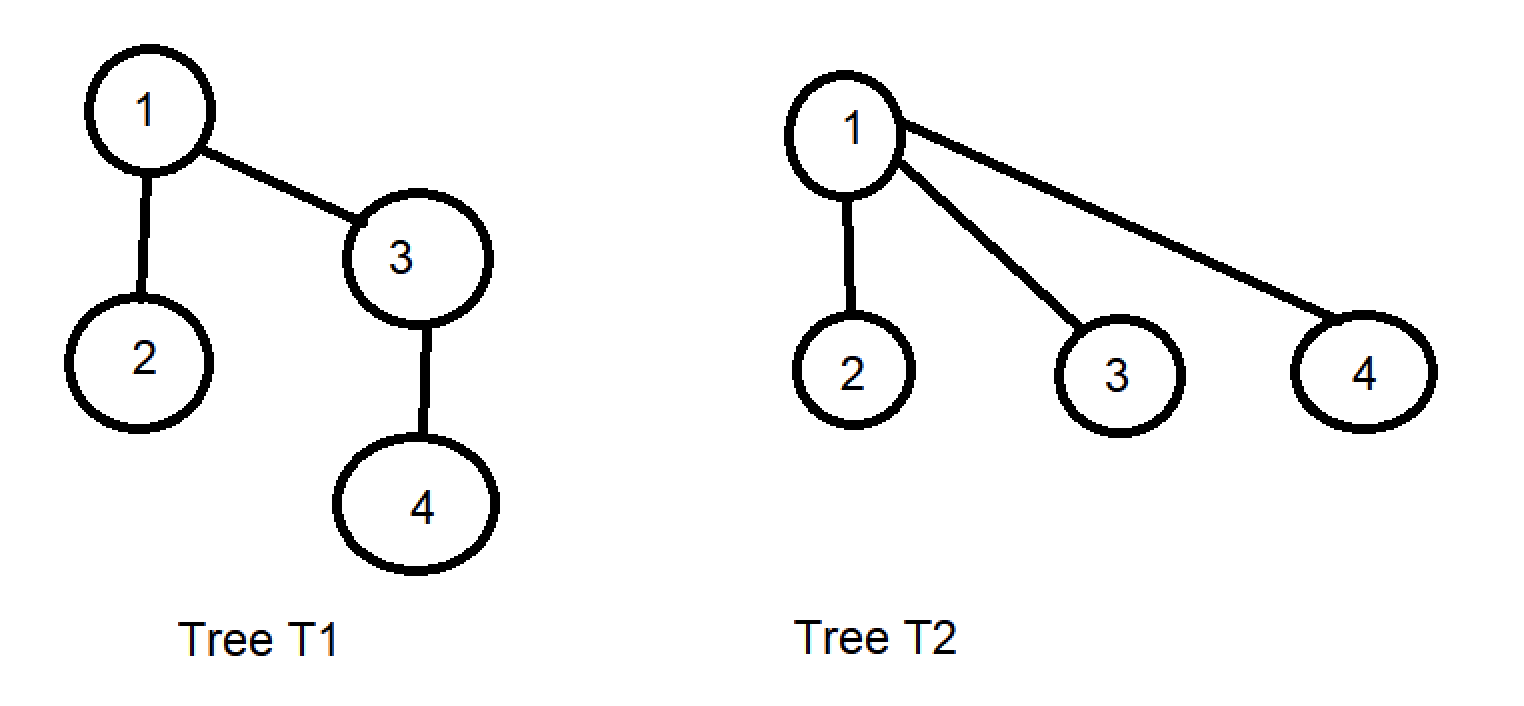
\includegraphics[width=8cm]{Question1a.png}
    \caption{Tree $T_1$ and $T_2$ are drawn differently due to path compression.}
    \label{fig:tree}
\end{figure}

\item The difference between $T_1$ and $T_2$ is that $T_1$ has no path compression while $T_2$ does. The smallest $n$ for which $T_1$ and $T_2$ are not equal is 8. Consider two empty trees $T_1$ and $T_2$. The first 4 operations are MAKE-SET(1), MAKE-SET(2), MAKE-SET(3), and MAKE-SET(4) (it doesn't have the be the numbers 1-4 but we choose these without loss of generality). Then we have UNION(1,2) and UNION(3,4) as the 5th and 6th operations. After that, we have UNION(1,3), to have one tree. At this point, both $T_1$ and $T_2$ are equivalent. Finally, for our 8th operation we have FIND-SET(4). At this point, the operation returns 1 as the answer for both $T_1$ and $T_2$ but due to path compression in $T_2$, the node containing 4 will no longer be connected to the node containing 3, but rather to the node containing 1 directly, because the node containing 1 is the representative. Thus, while $T_1$ and $T_2$ containing the same elements, after the 8th operation, they will be drawn differently (see Figure 1). Note that we choose to go with a tree with 4 nodes, because if we had 1, then both trees would clearly be equivalent. If we had 2 nodes, both trees would be still be equivalent because path compression would not affect the tree. If we had 3 nodes, because the trees use union by weight, we would have $T_1$ and $T_2$ both being drawn as a tree with one node as the representative and the other two nodes being connected to representative directly, meaning path compression would have no impact on $T_2$ when FIND-SET() was used. At 4 nodes, we can see the effects of path compression affecting the drawing of the $T_2$. Note, in this case path compression affects $T_2$ because when FIND-SET(4) is used, the pointer traverses from 4 to 3 to 1. So to speed up this process, path compression makes the node containing 4 point directly at the node containing 1. Thus, 8 is the smallest $n$ for which $T_1$ and $T_2$ are not equal.   


\item The difference between $T_2$ and $T_3$ is that $T_2$ is union by weight while $T_3$ is union by rank. To see the difference we need to use the UNION() function on two trees, where one has a greater weight but lower rank, and the other has a lower weight but higher rank. Clearly one node is not enough, as UNION() cannot be used. Two nodes is not enough, since both union by weight and by rank will result in the same tree. Likewise for three nodes, we would have a 2/1 split but one tree has a greater weight and rank compared to the other. For four nodes, a 2/2 or 3/1 split both result in the same tree after UNION() is used again. For five nodes, a 3/2 split will result in two trees of the same rank (rank 1). For six nodes, a 3/3 split is equal so it will not work, a 4/2 split will have a tree with greater weight and/or rank. For seven nodes, a 4/3 split will have a tree with greater weight and rank. For eight nodes, 4/4 is equal and so will not work, 3/5 will result in a tree with greater weight and rank. For nine nodes, we have a 4/5 split with the tree with 4 nodes having a greater rank, and the tree with 5 nodes having a greater weight but lesser rank. So the first nine operations are MAKE-SET(i) where i = 1,...,9. For the 5-node tree we have the following four operations, UNION(1,2), UNION(1,3), UNION(1,4), UNION(1,5). So the 5-node tree has a weight of 5 and a rank of 1. For the 4-node tree we have the following three operations, UNION(6,7), UNION(8,9), UNION(6,8). This 4-node tree has a weight of 4 but a rank of 2, since the longest height goes from 6 to 8 to 9 (starting from the top). Then, for $T_2$ the union of both trees will occur by weight meaning UNION(1,6) will result in a tree with the node containing 6 pointing at the node containing 1, since the 5-node tree with 1 as the representative is heavier, so the 4-node tree is appended to the 5-node tree. For, $T_3$ the union of both trees will occur by rank meaning UNION(1,6) will result in a tree with the node containing 1 pointing at the node containing 6, since the 4-node tree with 6 as the representative has the greater rank, so the 5-node tree is appended to the 4-node tree. Thus, the smallest $n$ for which $T_2$ and $T_3$ are not equivalent would be \textbf{\underline{17}}. Note: other possible splits for each number of nodes were not mentioned because they would not work for obvious reasons (e.g. splitting 8 nodes into 7/1 because then one tree would have a greater weight and rank than the other).

\end{enumerate}

\end{document}
